\section{Secure Software / Software Security}

Durch das Aufkommen des Internets nahm auch die vom \textit{National Institute of Standards and Technology} (NIST) erfassten Vulnerabilities mit hohem Ausmass zu.

\subsection{Most Dangerous Software Errors}
Die 25 häufigsten Schwachstellen können in drei Kategorien eingeteilt werden:
\begin{itemize}
	\item Ausgelöst durch unsichere Wege, in denen die Daten gesendet und empfangen werden. Dazu zählen \textit{SQL Injection}, \textit{OS Command Injection}, \textit{XSS}, \textit{CSRF} und \textit{Open Redirect}.
	\item Ausgelöst durch die unsichere Handhabung von Systemressourcen. Dazu gehören \textit{Classic Buffer Overflow}, \textit{Path Traversal}, \textit{Uncontrolled Format String}, \textit{Potentially Dangerous Function} und \textit{Integer Overflow}.
	\item Ausgelöst durch falsche Verwendung, Missbrauch oder Ignorierung von defensiven Sicherheitsmechanismen. Dazu zählen \textit{Missing Authentication}, \textit{Missing/Incorrect Authorization}, \textit{Hard-Coded Credentials}, \textit{Missing Encryption}, \textit{Reliance on Untrusted Inputs}, \textit{Incorrect Permission Assignment}, \textit{Use of broken or risky Cryptographic algorithm} und \textit{One-Way Hash without Salt}.
\end{itemize}

\subsection{Trinity of Trouble}
Folgende drei Aspekte sind mitunter verantwortlich für diese Schwierigkeiten.
\begin{description}
	\item[Connectivity] Immer mehr Systeme sind über das Internet miteinander verbunden und eröffnen somit neue \textit{Attack Vectors}. \textit{Service Oriented Architecture (SOA)} führt alte Systeme, welche nicht für die Vernetzung vorgesehen wurden, zusammen und veröffentlicht diese.
	\item[Extensibility] Systeme sind erweiterbar, wodurch ein teil der Kontrolle abgegeben wird. Über schlecht gewartete Erweiterungen können so neue Schwachstellen entstehen.
	\item[Complexity] Moderne Software wird immer komplexer. Mit dem Umfang nimmt auch die Fehlerrate quadratisch zu.
\end{description}

\subsection{Bugs + Flaws = Defects}
\begin{description}
	\item[Security Bug] Implementation-level Schwachstelle
	\item[Security Flaw] Design-level Schwachstelle (können selten automatisiert erkannt werden)
	\item[Security Defect] Ruhender defekt in der Software, welcher durch ein Bug oder Flaw ausgelöst wird.
\end{description}

\subsection{Software Artefakte}
Es gibt ein gemeinsames Set von Artefakten, welche unabhängig vom eigentlichen Entwicklungsprozess (Scrum, RUP, XP, \ldots) sind. Diese sind:
\begin{easylist}[itemize]
	& Anforderungen und Use Cases
	& Architektur und Design
	& Testpläne
	& Code
	& Tests und Testresultate
	& Rückmeldung von Kunden
\end{easylist}

\subsection{Drei Säulen der Software Security}

Zu den zentralen drei Säulen gehören \textbf{Risiko Management}, \textbf{Best Practices} und \textbf{Fachwissen}.

\subsubsection{Risiko Management}
Man identifiziert die betroffenen Personen, die technischen Risiken, auch die für das Unternehmen, und priorisiert sie anhand der gewonnenen Informationen. Danach kann eine Strategie zur Minderung entwickelt werden. Nach der Anwendung sollten die Anpassungen auf ihre Wirkung hin überprüft werden.

\begin{figure}[H]
	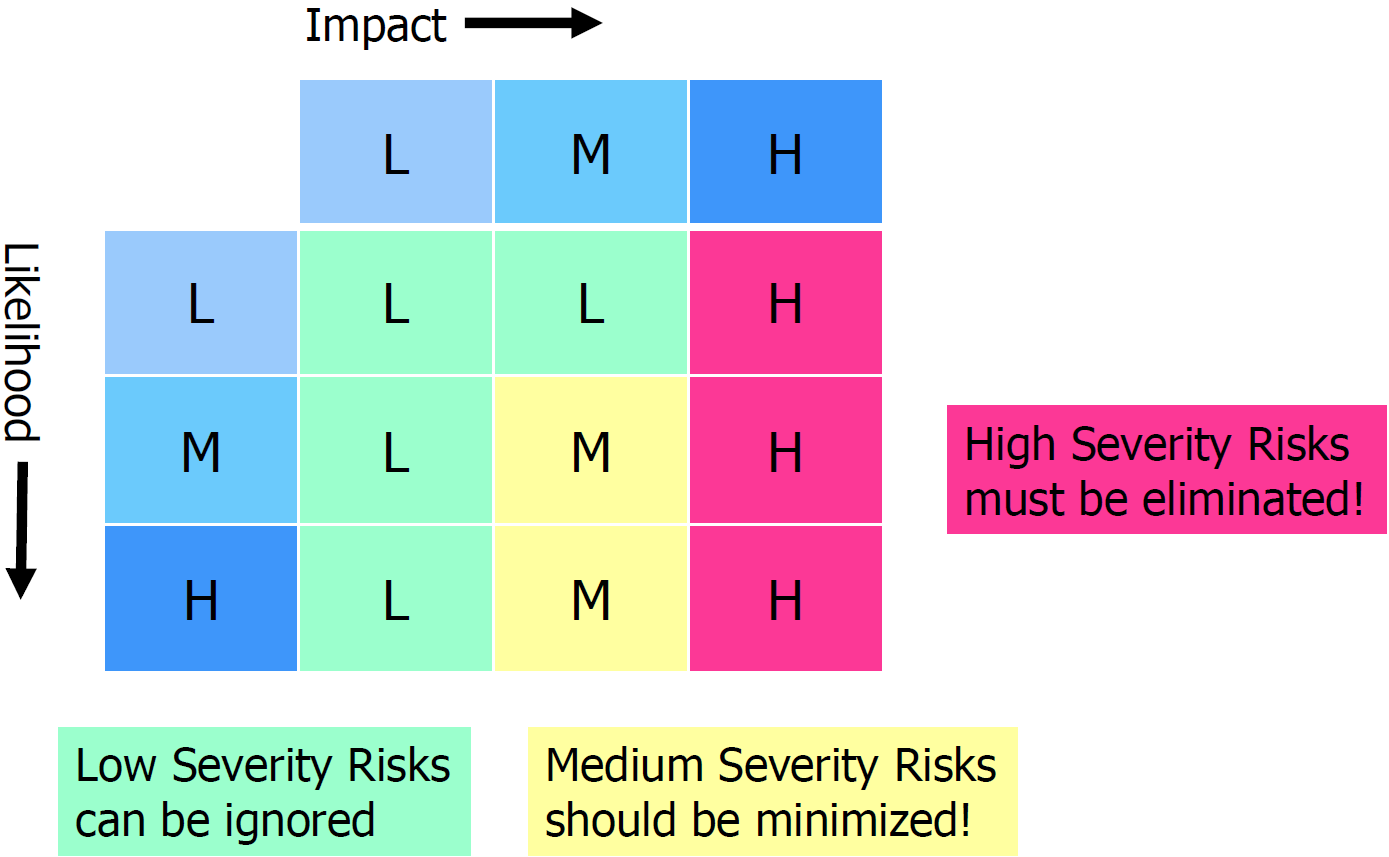
\includegraphics[width=0.6\textwidth]{./img/risk-evaluation}
	\caption{Risiko Evaluations-Matrix}
\end{figure}

\subsubsection{Best Practices}

Es folgen einige Best Practices in der Reihenfolge ihrer Effektivität. Sie können den Kategorien \textbf{K}onstruktiv (white hat) und \textbf{D}estruktiv (black hat) zugeordnet werden.
\begin{easylist}
	& Code Review \textbf{K}
	& Architectural risk analysis (historical knowledge) \textbf{K D}
	& Penetration testing \textbf{D}
	& Risk-based security tests \textbf{D K}
	& Abuse cases \textbf{D K}
	& Security requirements \textbf{K}
	& Security operation \textbf{K}
\end{easylist}

\subsubsection{Fachwissen}
Zum Fachwissen gibt es mehrere Perspektiven. Das Wissen über die Prinzipien, Rahmenbedingungen und Regeln gehören zum Vorgeschriebenen Fachwissen. Dazu gesellt sich die Diagnostischen Fähigkeiten mit dem Wissen über Angriffe, Schwachstellen und Angriffsmuster. Zuletzt benötigt man auch ein Wissen über die Vergangenheit.

\begin{figure}[H]
	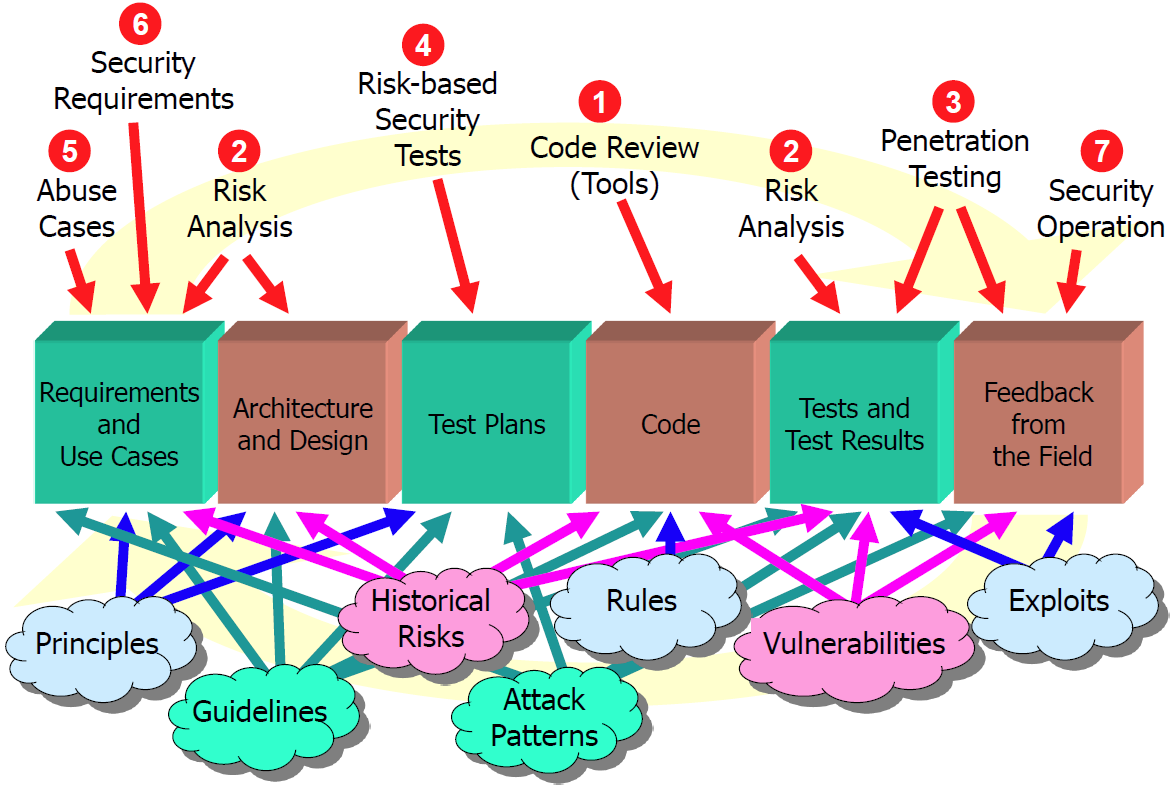
\includegraphics[width=\textwidth]{./img/sdl-best-practice}
	\caption{Best Practices und Fachwissen angewendet auf die Software Artefakte}
\end{figure}

\subsection{Code Analyse}

Für die Analyse von Sourcecode bieten sich mehrere Lösungen an, welche den Quellcode und auch das laufende Programm analysieren und auswerten können. Die ersten Generationen von solchen Analyseprogrammen wurden auch als \textit{Intelligentes Grep} bezeichnet und lieferten viele false positives. In späteren, oft kommerziellen Tools, wurden diese, durch Parsen des Source-Codes, versucht zu minimieren.

Das Wissen aus der Vergangenheit ist in die Regelsätze dieser Software eingeflossen. Jedoch können Probleme in der Softwarearchitektur nicht oder nur selten erkannt werden. Ein manuelles Review ist somit weiterhin nötig. Auch können Abhängigkeiten und falsche Benutzung externer Komponenten nicht korrekt überprüft und erkannt werden.

\todo[inline]{Code-Analyse}
\todo[inline]{SDL}